\documentclass[black,white]{beamer}

\usepackage{beamerthemesplit}
\usepackage{epstopdf}
\usepackage{graphicx}
\usepackage{subfigure}
\usepackage{hyperref}
\usepackage[utf8]{inputenc}
\usepackage[english]{babel}
\usepackage{listings}
\usepackage{array}
\usepackage{color}
\usepackage{colortbl}

\usefonttheme{professionalfonts}
\usecolortheme{dove}
\useoutertheme{infolines}
\useinnertheme{rectangles}

\setlength{\parindent}{0pt}
\newcommand*\sfb[1]{\textbf{#1}}
\definecolor{red2}{rgb}{.7,0,.39}
\setbeamercolor{title}{fg=white}
\setbeamercolor{frametitle}{fg=white}
\setbeamercolor{framesubtitle}{fg=white}
\setbeamercolor{normal text}{fg=white}
\usebackgroundtemplate{
	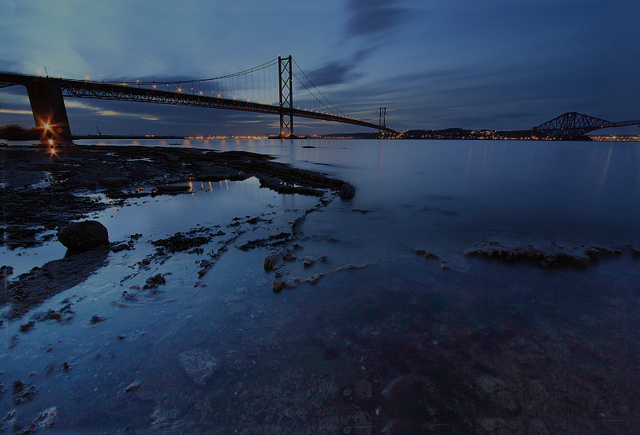
\includegraphics[width=\paperwidth,height=\paperheight]{img/bg.jpg}
}

\begin{document}

\title[netyack / the telephony network]{\huge{On creating a novel, future
					      global telephony network}}
\author[Daniel Borkmann] {
	\vspace*{-20pt}
	\newline
	Daniel Borkmann	\texttt{<dborkma@tik.ee.ethz.ch>}\\
	\texttt{http://gnumaniacs.org}\\\bigskip
	IET PATW 2011, Switzerland
}
\institute [ETH Zurich]{}
\date[\today]{}

\frame {
	\titlepage
}


\section{Basics of ANA}
\frame {
	\frametitle{\textcolor{red2}{ETH Zurich}}
}

\end{document}

